\documentclass[journal,12pt,twocolumn]{IEEEtran}

\usepackage{setspace}
\usepackage{gensymb}
\singlespacing
\usepackage[cmex10]{amsmath}

\usepackage{amsthm}

\usepackage{mathrsfs}
\usepackage{txfonts}
\usepackage{stfloats}
\usepackage{bm}
\usepackage{cite}
\usepackage{cases}
\usepackage{subfig}

\usepackage{longtable}
\usepackage{multirow}
\usepackage{enumitem}
\usepackage{mathtools}
\usepackage{steinmetz}
\usepackage{tikz}
\usepackage{circuitikz}
\usepackage{verbatim}
\usepackage{tfrupee}
\usepackage[breaklinks=true]{hyperref}
\usepackage{graphicx}
\usepackage{tkz-euclide}

\usetikzlibrary{calc,math}
\usepackage{listings}
    \usepackage{color}                                            %%
    \usepackage{array}                                            %%
    \usepackage{longtable}                                        %%
    \usepackage{calc}                                             %%
    \usepackage{multirow}                                         %%
    \usepackage{hhline}                                           %%
    \usepackage{ifthen}                                           %%
    \usepackage{lscape}     
\usepackage{multicol}
\usepackage{chngcntr}

\DeclareMathOperator*{\Res}{Res}

\renewcommand\thesection{\arabic{section}}
\renewcommand\thesubsection{\thesection.\arabic{subsection}}
\renewcommand\thesubsubsection{\thesubsection.\arabic{subsubsection}}

\renewcommand\thesectiondis{\arabic{section}}
\renewcommand\thesubsectiondis{\thesectiondis.\arabic{subsection}}
\renewcommand\thesubsubsectiondis{\thesubsectiondis.\arabic{sub subsection}}


\hyphenation{optical networks semiconduc-tor}
\def\inputGnumericTable{}                                 %%

\lstset{
%language=C,
frame=single, 
breaklines=true,
columns=fullflexible
}
\date{March 2021}

\begin{document}

\newtheorem{theorem}{Theorem}[section]
\newtheorem{problem}{Problem}
\newtheorem{proposition}{Proposition}[section]
\newtheorem{lemma}{Lemma}[section]
\newtheorem{corollary}[theorem]{Corollary}
\newtheorem{example}{Example}[section]
\newtheorem{definition}[problem]{Definition}
\newcommand{\BEQA}{\begin{eqnarray}}
\newcommand{\EEQA}{\end{eqnarray}}
\newcommand{\define}{\stackrel{\triangle}{=}}
\bibliographystyle{IEEEtran}
\raggedbottom
\setlength{\parindent}{0pt}
\providecommand{\mbf}{\mathbf}
\providecommand{\pr}[1]{\ensuremath{\Pr\left(#1\right)}}
\providecommand{\qfunc}[1]{\ensuremath{Q\left(#1\right)}}
\providecommand{\fn}[1]{\ensuremath{f\left({#1}\right)}}
\providecommand{\e}[1]{\ensuremath{E\left(#1\right)}}
\providecommand{\sbrak}[1]{\ensuremath{{}\left[#1\right]}}
\providecommand{\lsbrak}[1]{\ensuremath{{}\left[#1\right.}}
\providecommand{\rsbrak}[1]{\ensuremath{{}\left.#1\right]}}
\providecommand{\brak}[1]{\ensuremath{\left(#1\right)}}
\providecommand{\lbrak}[1]{\ensuremath{\left(#1\right.}}
\providecommand{\rbrak}[1]{\ensuremath{\left.#1\right)}}
\providecommand{\cbrak}[1]{\ensuremath{\left\{#1\right\}}}
\providecommand{\lcbrak}[1]{\ensuremath{\left\{#1\right.}}
\providecommand{\rcbrak}[1]{\ensuremath{\left.#1\right\}}}
\theoremstyle{remark}
\newtheorem{rem}{Remark}
\newcommand{\sgn}{\mathop{\mathrm{sgn}}}
\newcommand{\comb}[2]{{}^{#1}\mathrm{C}_{#2}}
\providecommand{\abs}[1]{\vert#1\vert}
\providecommand{\res}[1]{\Res\displaylimits_{#1}} 
\providecommand{\norm}[1]{\lVert#1\rVert}
%\providecommand{\norm}[1]{\lVert#1\rVert}
\providecommand{\mtx}[1]{\mathbf{#1}}
\providecommand{\mean}[1]{E\sbrak{ #1 }}
\providecommand{\fourier}{\overset{\mathcal{F}}{ \rightleftharpoons}}
%\providecommand{\hilbert}{\overset{\mathcal{H}}{ \rightleftharpoons}}
\providecommand{\system}{\overset{\mathcal{H}}{ \longleftrightarrow}}
	%\newcommand{\solution}[2]{\textbf{Solution:}{#1}}
\newcommand{\solution}{\noindent \textbf{Solution: }}
\newcommand{\cosec}{\,\text{cosec}\,}
\providecommand{\dec}[2]{\ensuremath{\overset{#1}{\underset{#2}{\gtrless}}}}
\newcommand{\myvec}[1]{\ensuremath{\begin{pmatrix}#1\end{pmatrix}}}
\newcommand{\mydet}[1]{\ensuremath{\begin{vmatrix}#1\end{vmatrix}}}
\numberwithin{equation}{subsection}
\makeatletter
\@addtoreset{figure}{problem}
\makeatother
\let\StandardTheFigure\thefigure
\let\vec\mathbf
\vspace{3cm}
\title{EE3900 Assignment - 3}
\author{Adhvik Mani Sai Murarisetty - AI20BTECH11015}
\maketitle
\newpage
\bigskip
\renewcommand{\thetable}{\theenumi}

Download latex-tikz codes from 
%
\begin{lstlisting}
https://github.com/adhvik24/EE3900/blob/main/Assignment3/Assignment3.tex
\end{lstlisting}
%
Download python codes from 
%
\begin{lstlisting}
https://github.com/adhvik24/EE3900/blob/main/Assignment3/Assignment3.py
\end{lstlisting}
\section{Ramsey 4.2 qn 15}
Find the zeroes of the quadratic polynomial
$x^2+7x+10$ and verify the relationship between
the zeroes and the coefficients.
\section{SOLUTION}

\begin{lemma}
A general polynomial equation $p(x,y)$ of degree 2 is given by :
\begin{align}
Ax^2 + Bxy + Cy^2 + Dx + Ey + F = 0
\end{align}
The vector equation of $p(x,y)$ is given by :
\begin{align}
\vec{x^T}\myvec{A & \frac{B}{2} \\ \frac{B}{2} & C}\vec{x} + \myvec{D & E}\vec{x} + F=0\label{eq:1}
\end{align}
And for a quadratic polynomial we have :
\begin{align}
B &= 0\\
C &= 0\\
E &= 0
\end{align}
If we take $A = 1$ , we have :
\begin{align}
\text{Sum of zeroes} = -D \\
\text{Product of zeroes} = F 
\end{align}

\end{lemma}

The given equation can be written as,
\begin{align}
    \vec{x}^T\myvec{1 & 0 \\ 0 & 0}\vec{x} + \myvec{7 & 0}\vec{x} + 10 = 0 \label{eq:2}
\end{align}
where,
\begin{align}
    \vec{x} = \myvec{x \\ 0} \label{eq:3}
\end{align}
Substituting \eqref{eq:3} in \eqref{eq:2},
\begin{align}
    \myvec{x \\ 0}^T\myvec{1 & 0 \\ 0 & 0}\myvec{x \\ 0} + \myvec{7 & 0}\myvec{x \\ 0} + 10 &= 0 
\end{align}
\begin{align}
    \implies x^2 + 7x + 10 &= 0\\
    \implies \brak{x + \frac{7}{2}}^2 &= \frac{9}{4}\\
    \implies \brak{x + \frac{7}{2}} &= \pm\frac{3}{2}\label{eq:4}\\
    \implies x  &= -2,-5\label{eq:5}
\end{align}

Verifying the relationship between the zeroes and coefficients. By comparing \eqref{eq:2} with \eqref{eq:1},
\begin{align}
    \implies \text{sum of the zeroes} = -7 = -D\\
    \text{product of zeroes} = 10 = F.
\end{align}

$\therefore$ The zeroes of equation $x^2+7x+10$ are -2, -5.
\begin{figure}
    \centering
    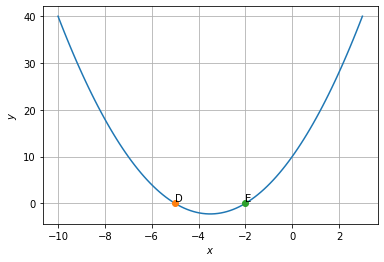
\includegraphics[width=\columnwidth]{a_5.png}
    \caption{Quadratic polynomial $x^2+7x+10$}
    \label{fig:my_label}
\end{figure}
\end{document}
